\section{Исследовательская часть}
Замеры времени работы CPU и ядер с различными конфигурациями проводятся на изображении с разрешением 640 на 480 пикселей без сглаживания. Здесь $k$ --- глубина рекурсии.

\resizebox{\columnwidth}{!}{
\begin{tabular}{|c|c|c|c|c|c|c|c|c|}
\hline
Общее& & & & \\
количество лучей & 307200 & 560757 & 961274 & 1763305 \\
\hline
Конфигурация & $k = 1$ & $k = 2$ & $k = 4$ & $k = 8$ \\
\hline
CPU & 2788.919 & 4580.225 & 8266.978 & 15293.571 \\
\hline
(1, 32) & 11456.789 & 22303.668 & 45185.785 & 94536.047 \\
\hline
(32, 32) & 415.182 & 797.055 & 1644.077 & 3496.258 \\
\hline
(256, 32) & 213.678 & 397.268 & 818.838 & 1745.377 \\
\hline
(256, 256) & 210.404 & 390.930 & 790.606 & 1693.551 \\
\hline
\end{tabular}
}

\subsection{Входные данные}
Входные данные, на которых получается наиболее красочный результат:
\begin{alltt}
225
./res/%d.data
1920 1080 120

4.0 0.0 0.0   1.0 1.0   1.0 1.0 1.0   0.0 0.0
2.0 0.0 0.0   0.5 0.1   1.0 1.0 1.0   0.0 0.0

 2.0  0.0  0.0    1.0  0.0  1.0   2.0    0.65   0.25   10
-1.5 -1.5  0.5    0.0  1.0  0.0   1.75   0.25   0.65   5
-1.0  3.0  0.75   0.75 0.75 0.0   1.5    0.45   0.45   2

-6.0 -6.0 -3.0   -6.0  6.0  0.0   6.0 6.0 -2.0   6.0 -6.0 -1.0
./textures/checkerboard.data 0.75 0.75 0.75 0.5

4
-5  5 4     1.0 0.5 0.0
-5 -5 2     0.0 1.0 0.0
 5 -5 1     0.0 0.0 1.0
 5  5 3     1.0 1.0 1.0

10 2
\end{alltt}

\section{Трёхмерные графики}
\begin{center}
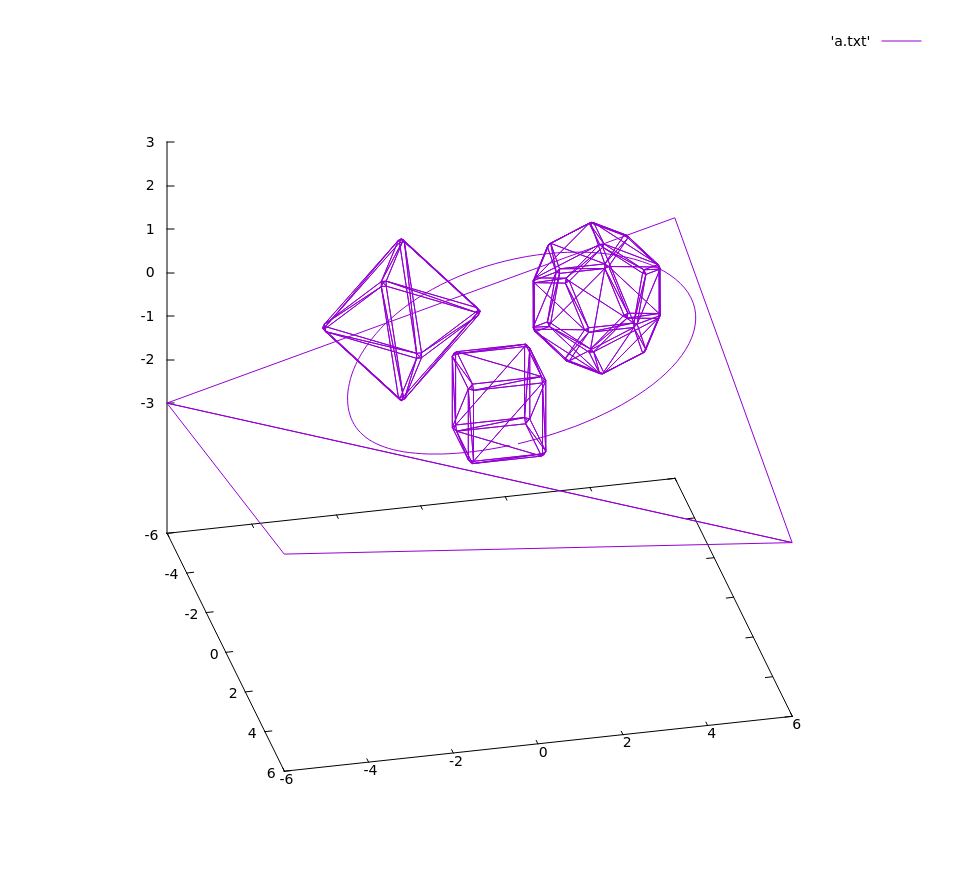
\includegraphics[width=\textwidth]{gnuplot1.png}\newline\noindent
Вид спереди
\end{center}
\pagebreak
\begin{center}
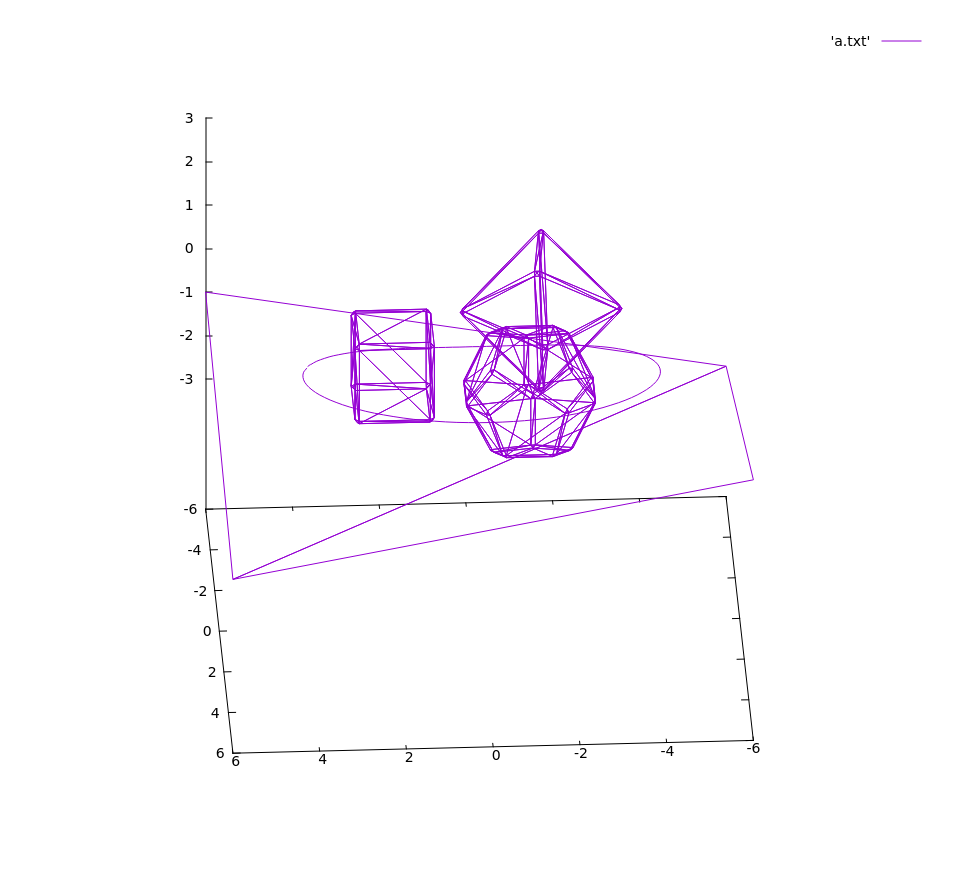
\includegraphics[width=\textwidth]{gnuplot2.png}\newline\noindent
Вид справа
\end{center}
\pagebreak
\begin{center}
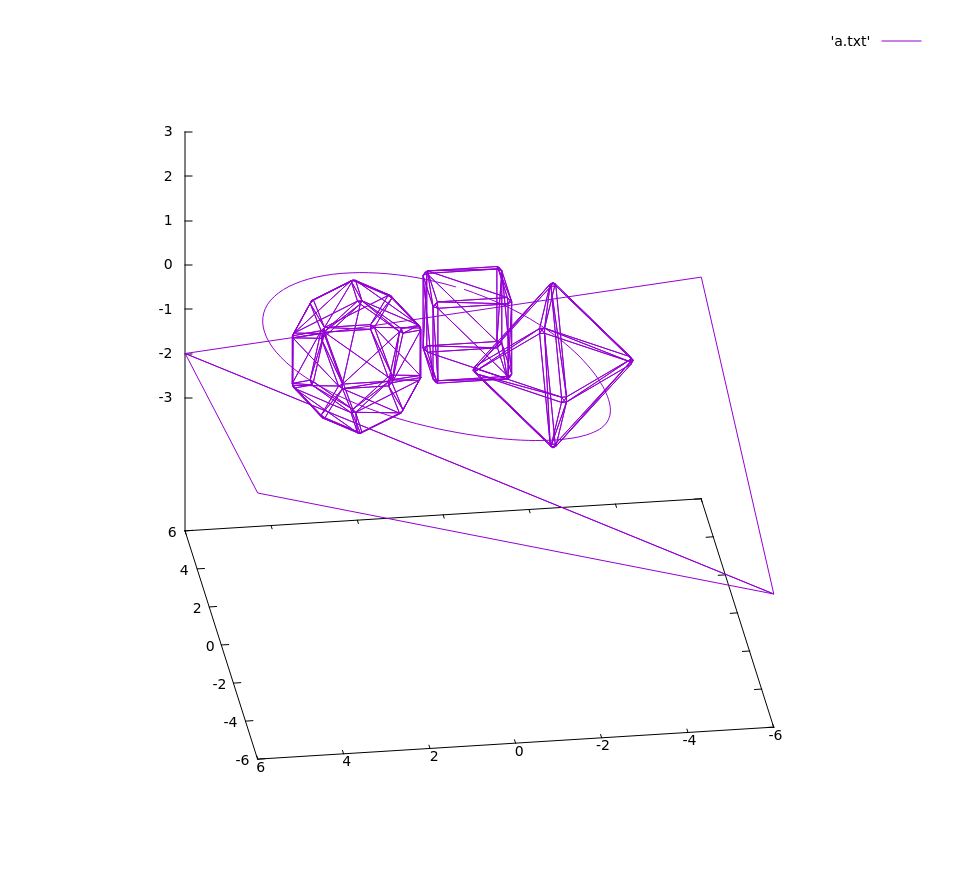
\includegraphics[width=\textwidth]{gnuplot3.png}\newline\noindent
Вид сзади
\end{center}
\pagebreak
\begin{center}
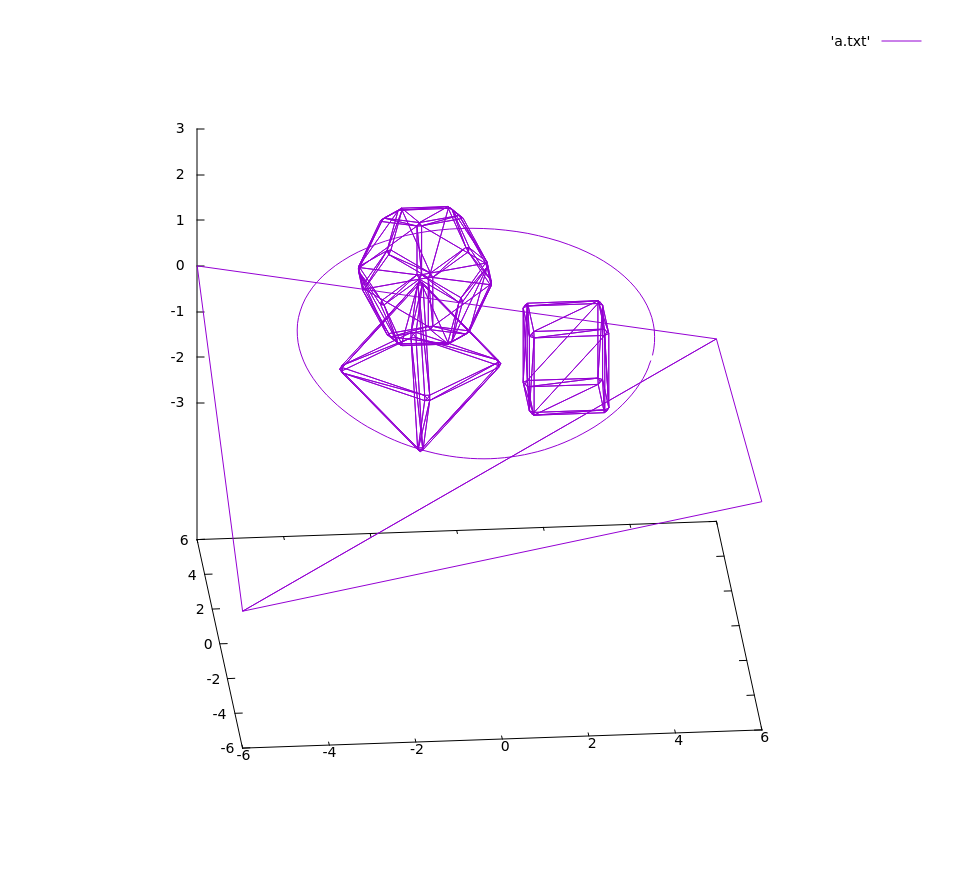
\includegraphics[width=\textwidth]{gnuplot4.png}\newline\noindent
Вид слева
\end{center}
\pagebreak

\section{Результаты}
\begin{center}
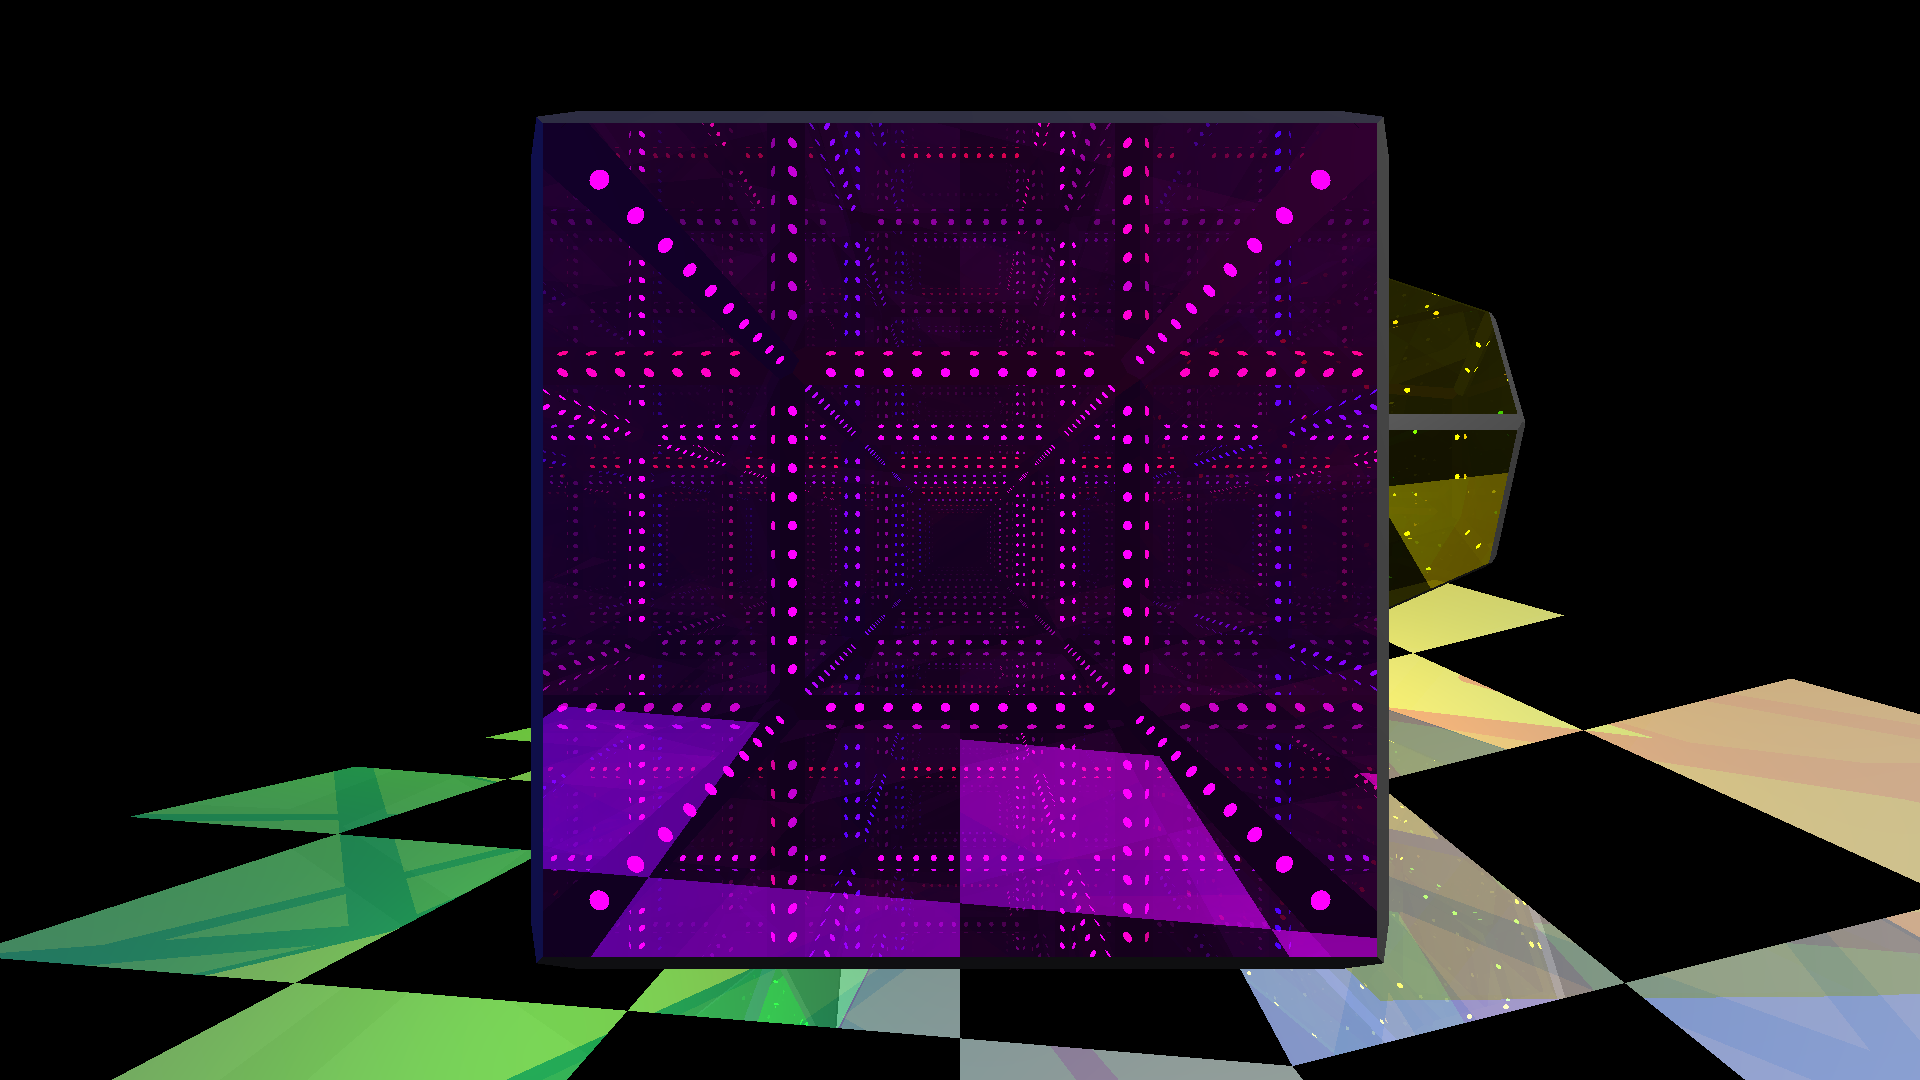
\includegraphics[width=\textwidth]{001.png}\newline\noindent
Эффект бесконечности в кубе
\end{center}
\begin{center}
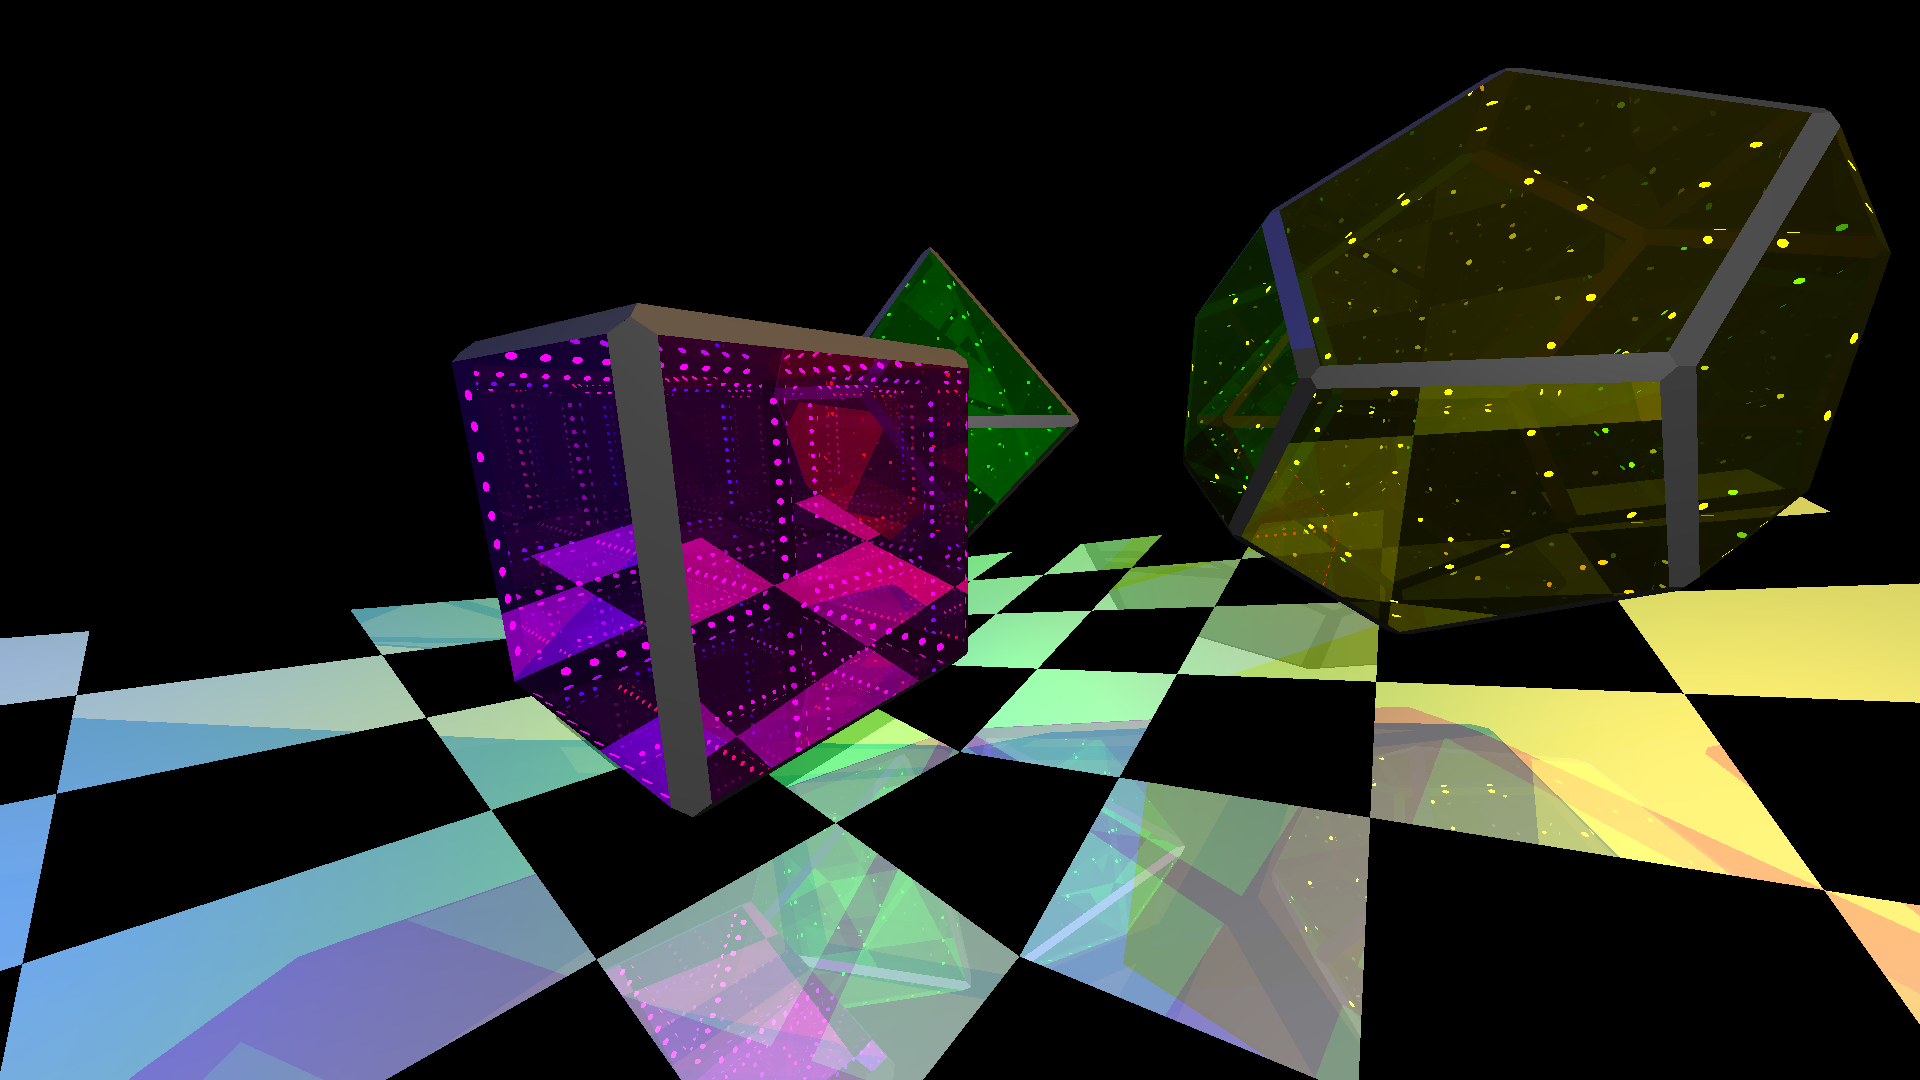
\includegraphics[width=\textwidth]{002.png}\newline\noindent
Два отражения октаэдра от пола
\end{center}
\pagebreak

\begin{center}
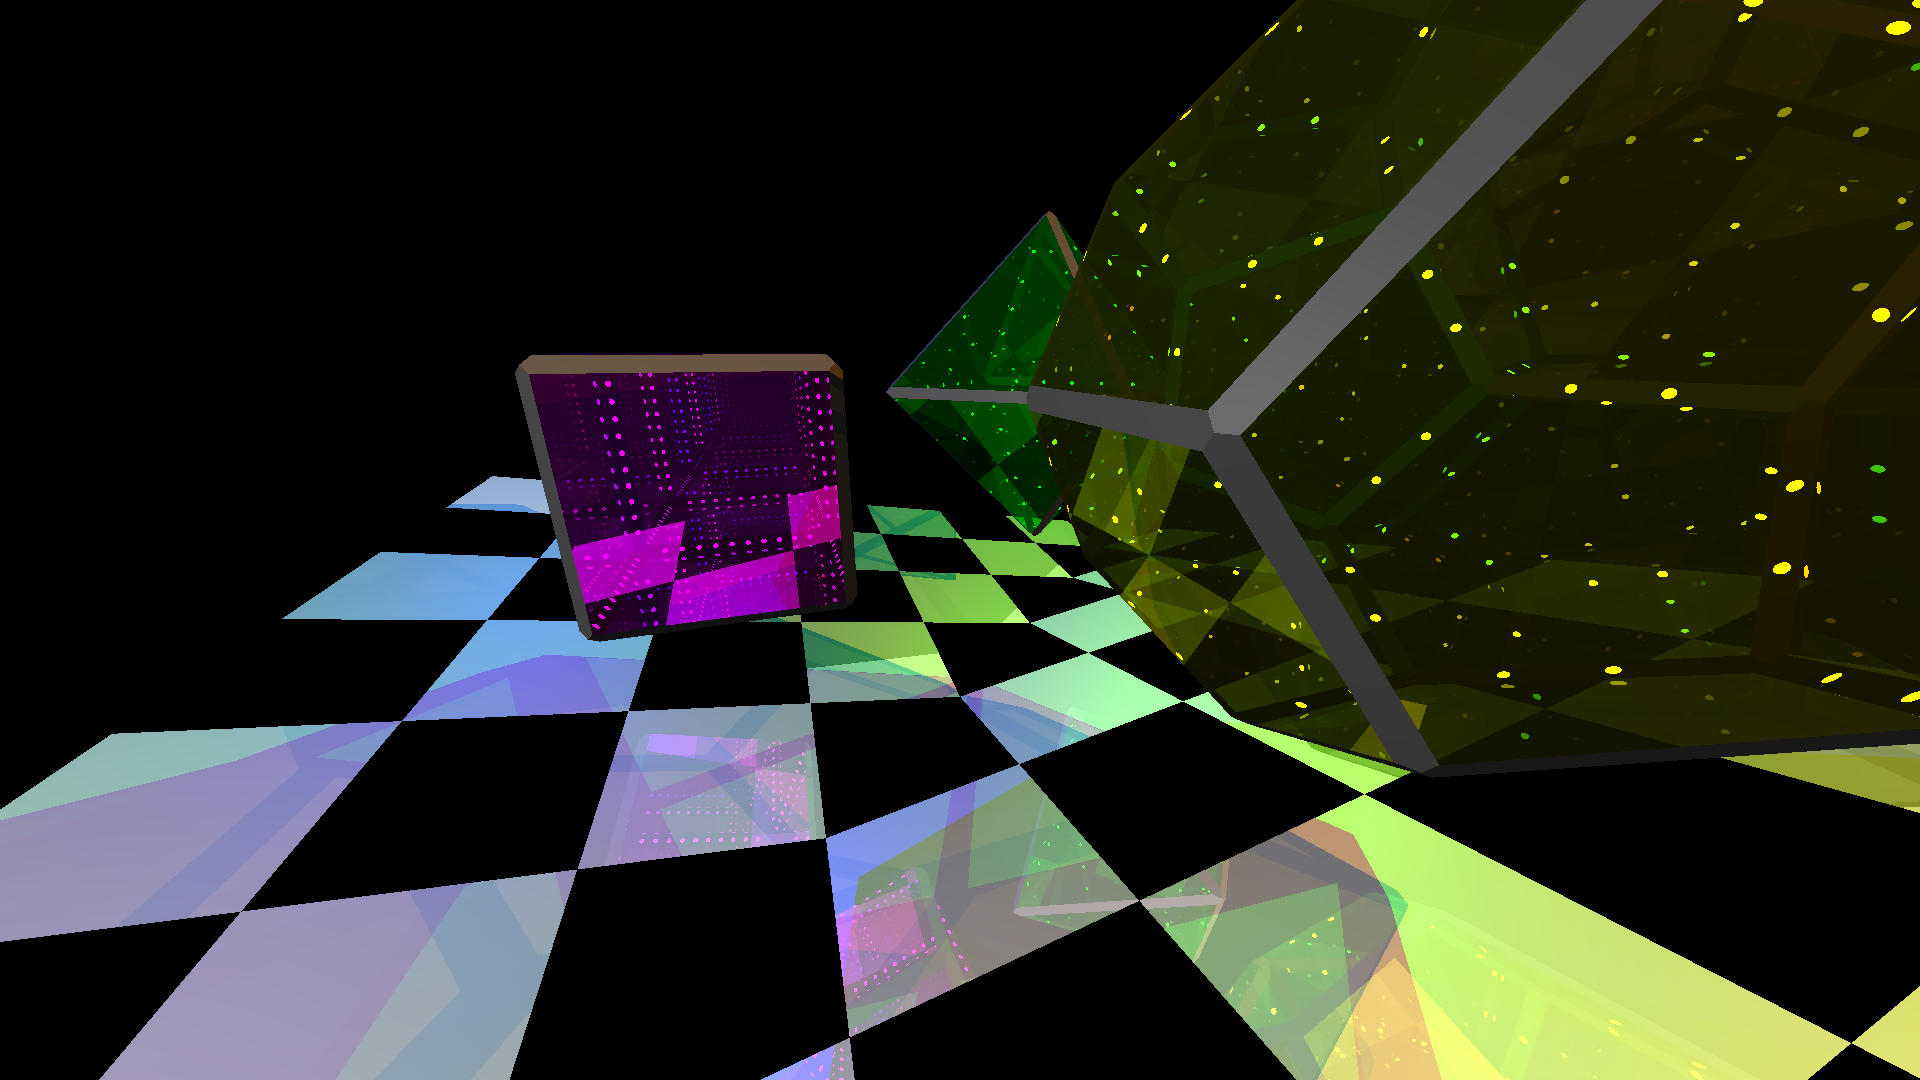
\includegraphics[width=\textwidth]{003.png}\newline\noindent
Октаэдр частично виден сквозь додекаэдр
\end{center}
\begin{center}
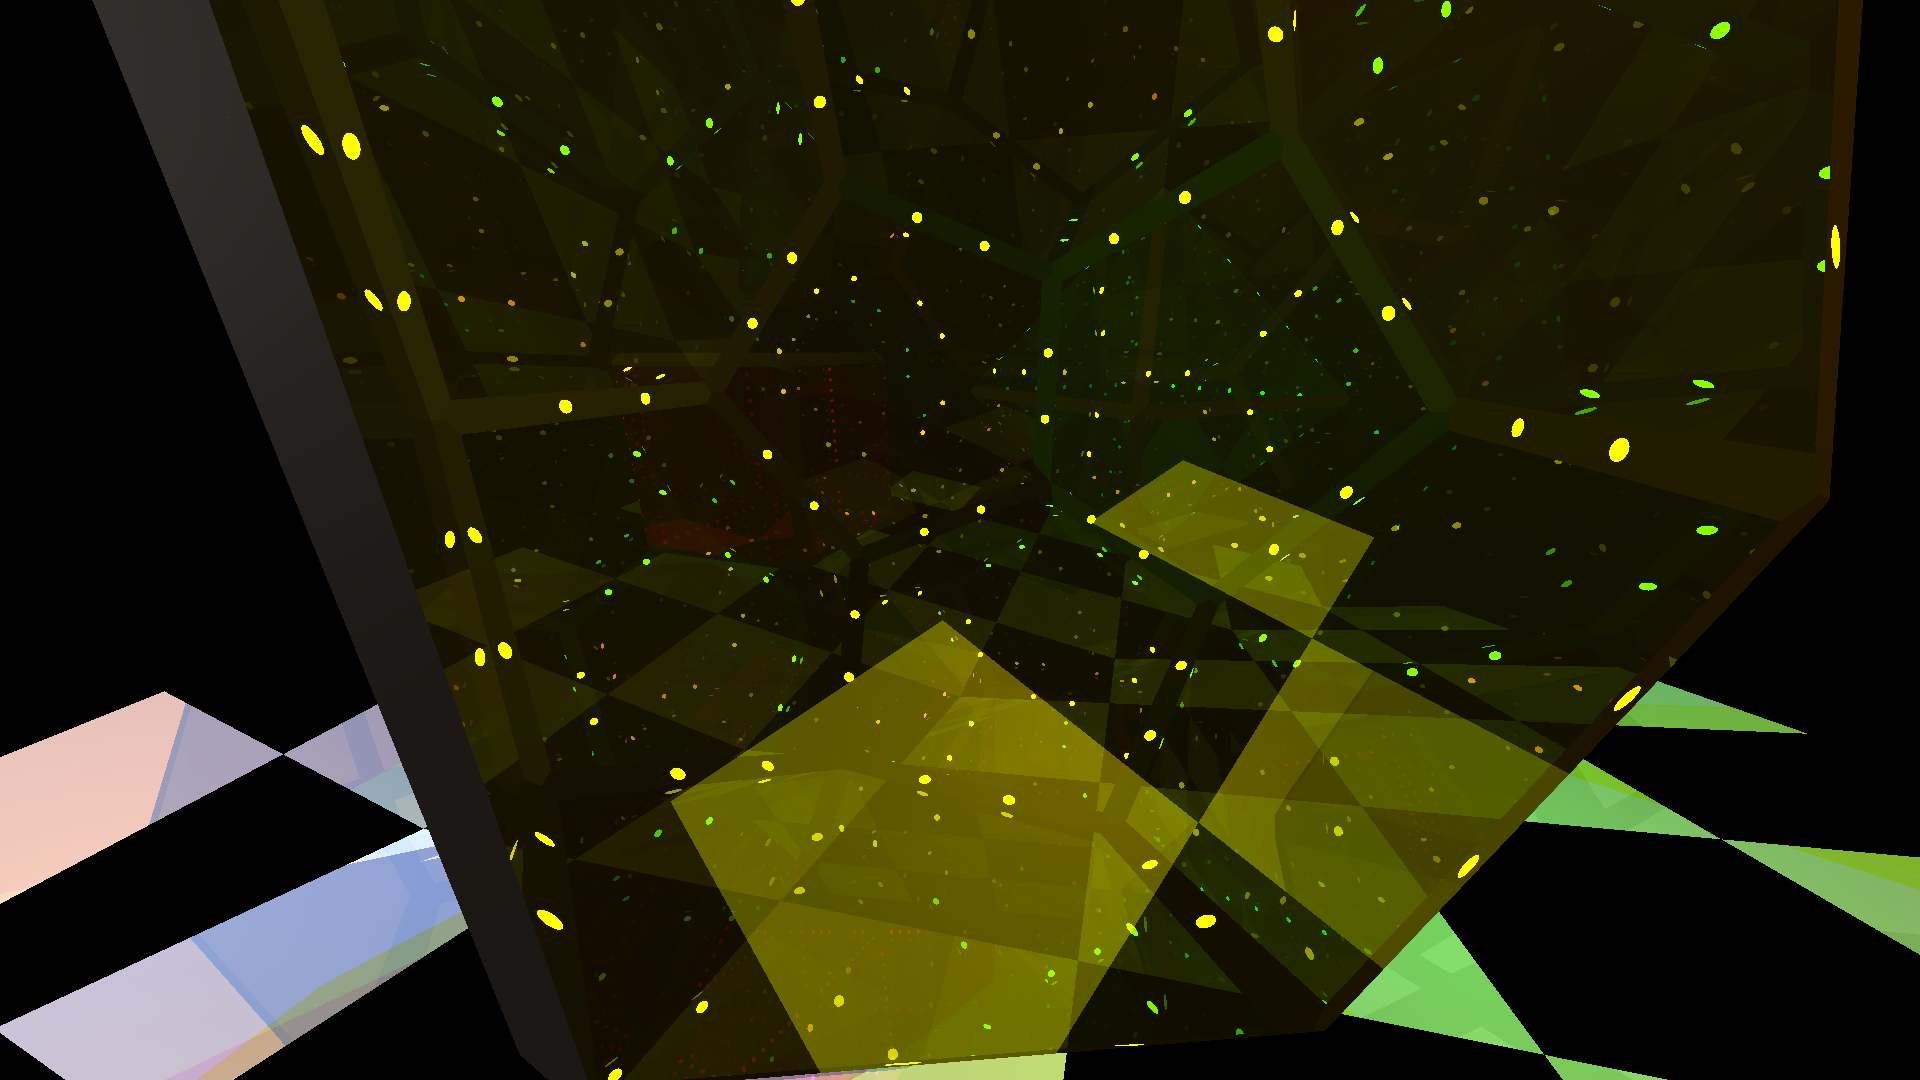
\includegraphics[width=\textwidth]{004.png}\newline\noindent
Эффект бесконечности в кубе в додекаэдре
\end{center}
\pagebreak

\begin{center}
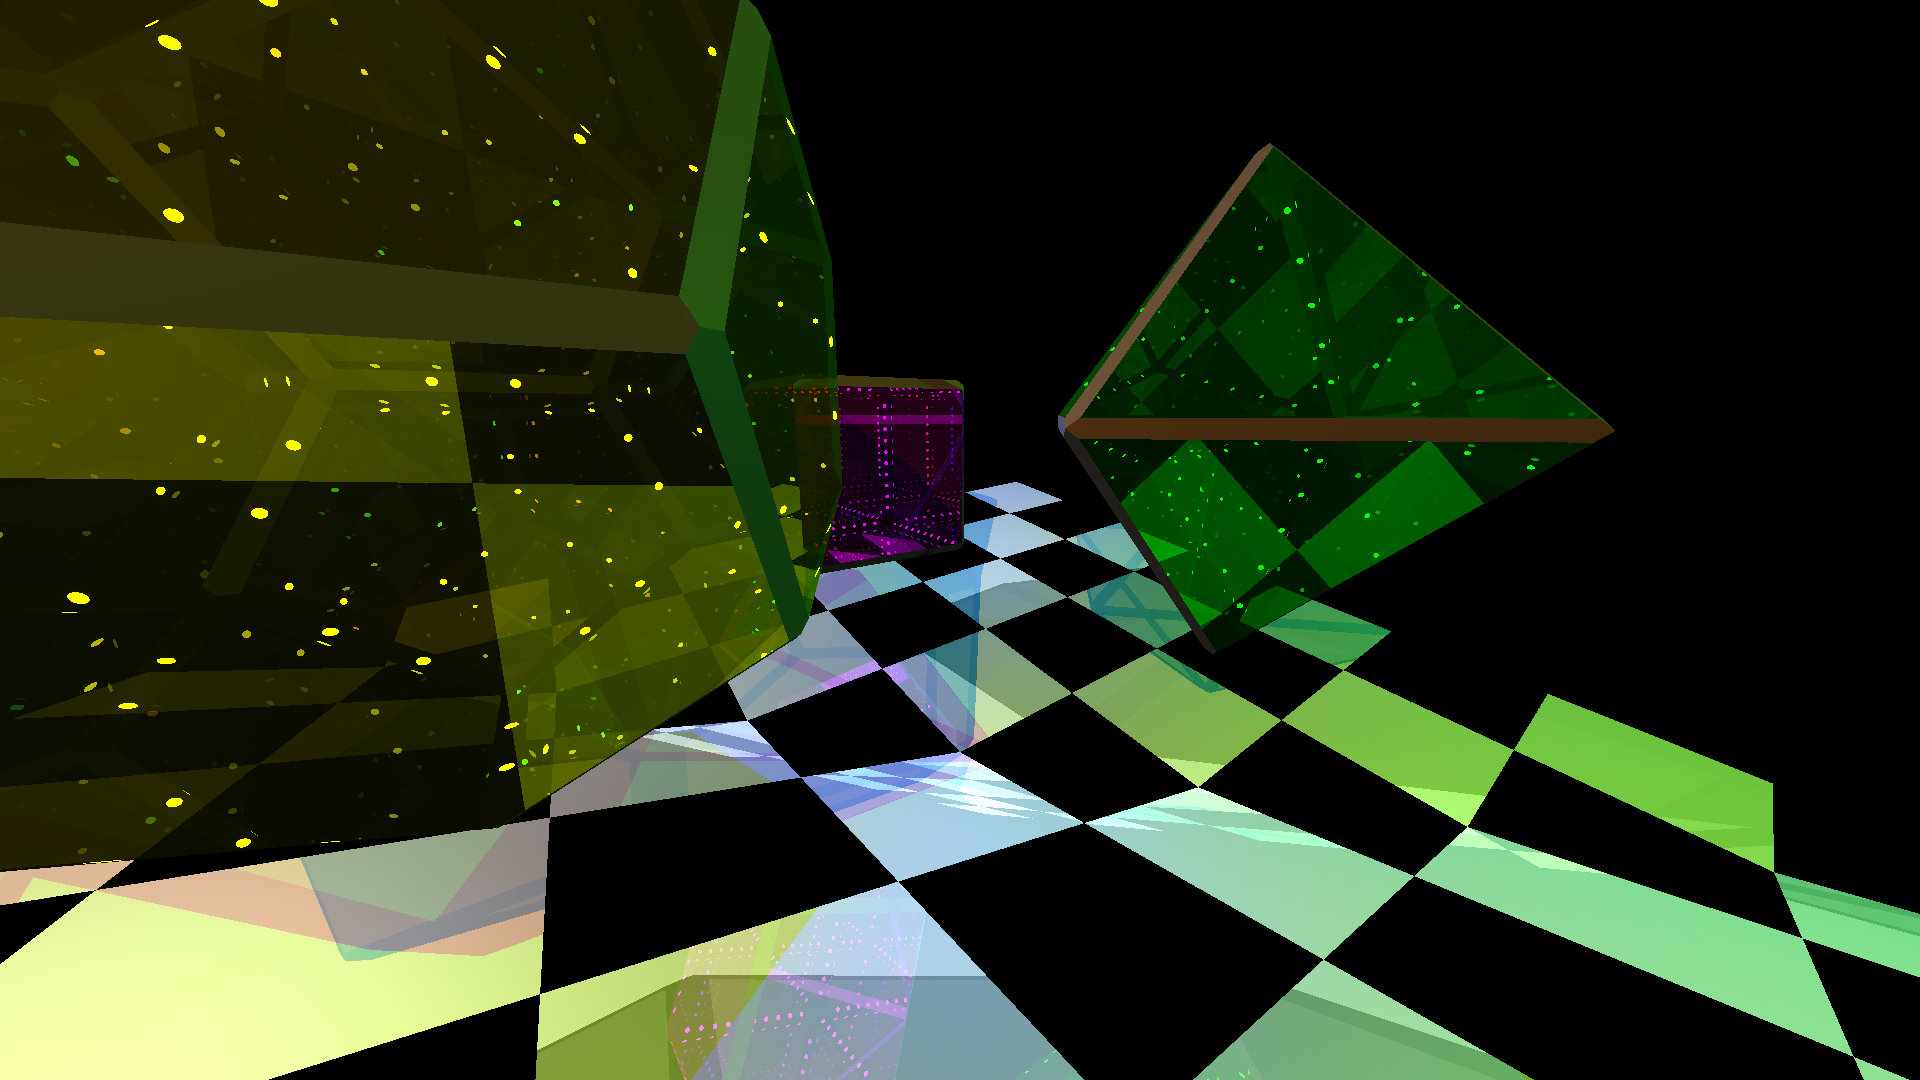
\includegraphics[width=\textwidth]{005.png}\newline\noindent
Отражение куба от пола
\end{center}
\begin{center}
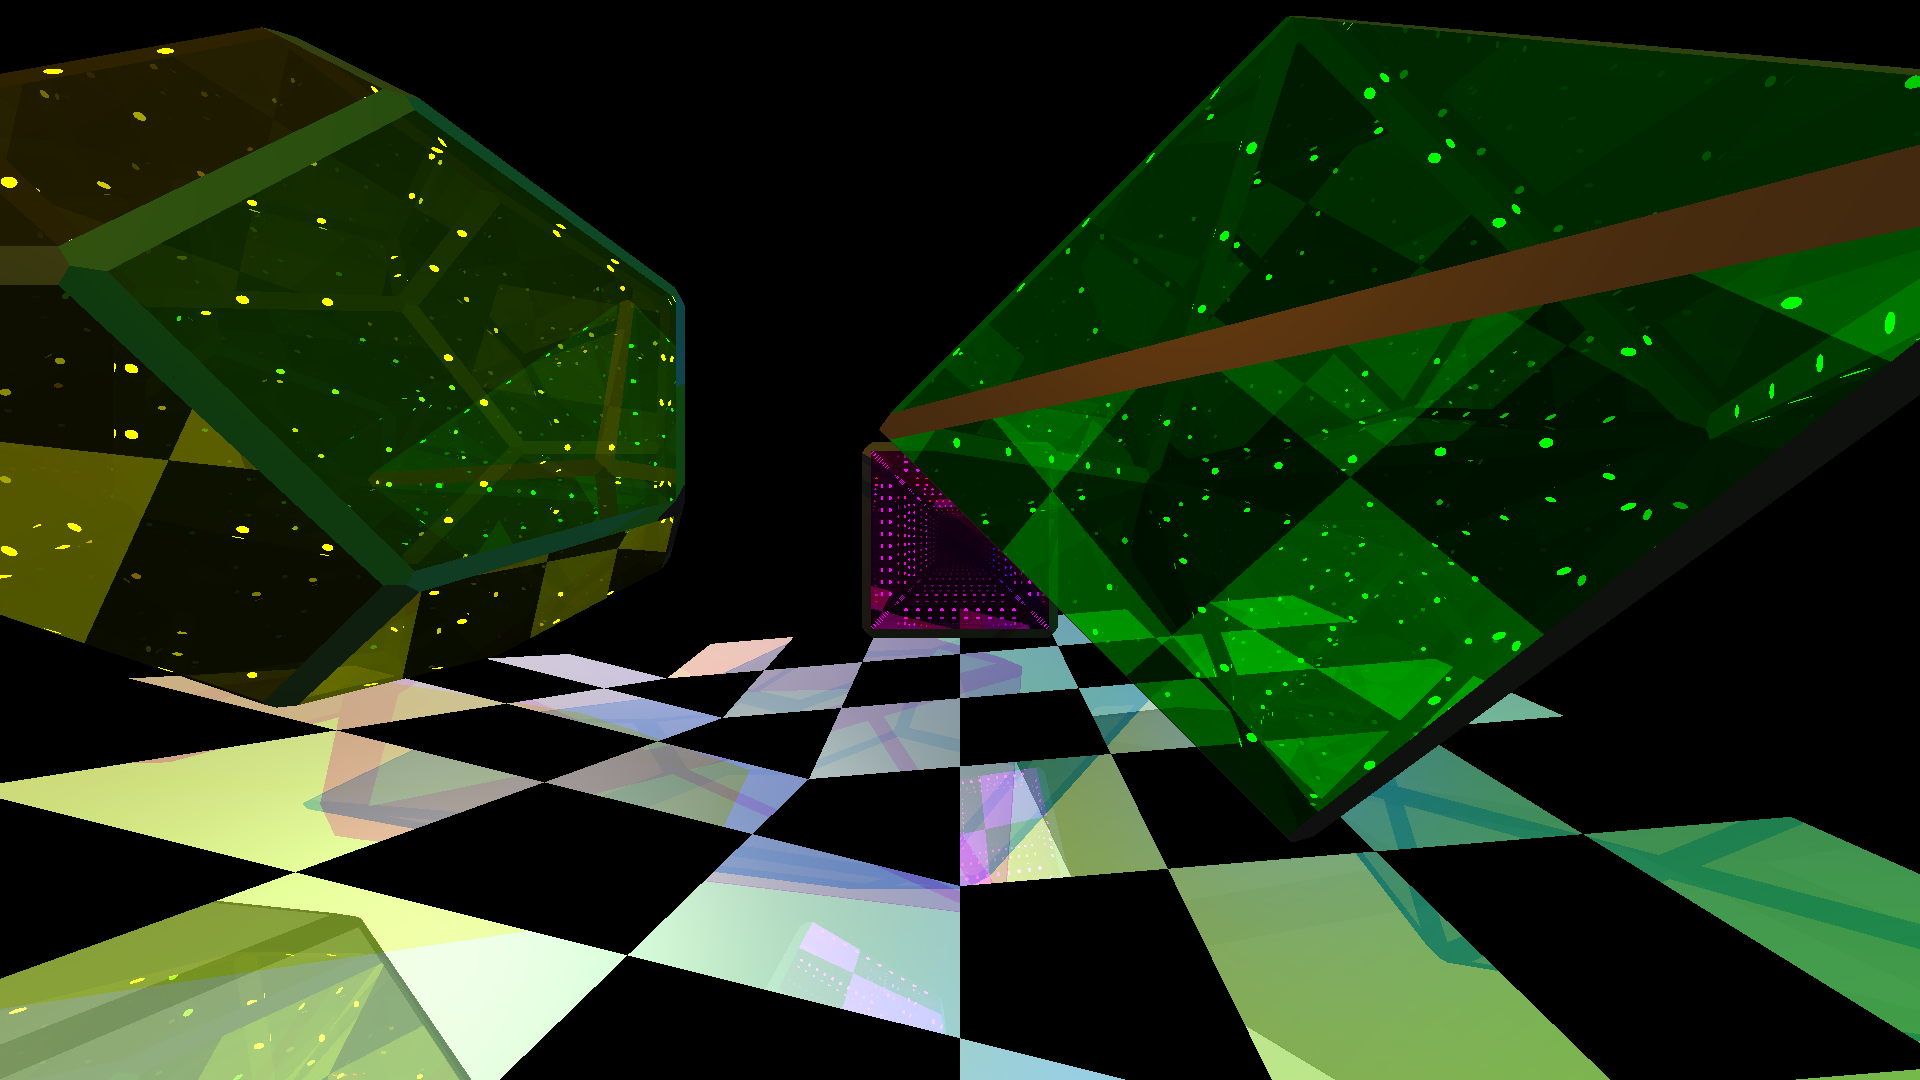
\includegraphics[width=\textwidth]{006.png}\newline\noindent
Октаэдр отражается в додекаэдре
\end{center}
\pagebreak

\begin{center}
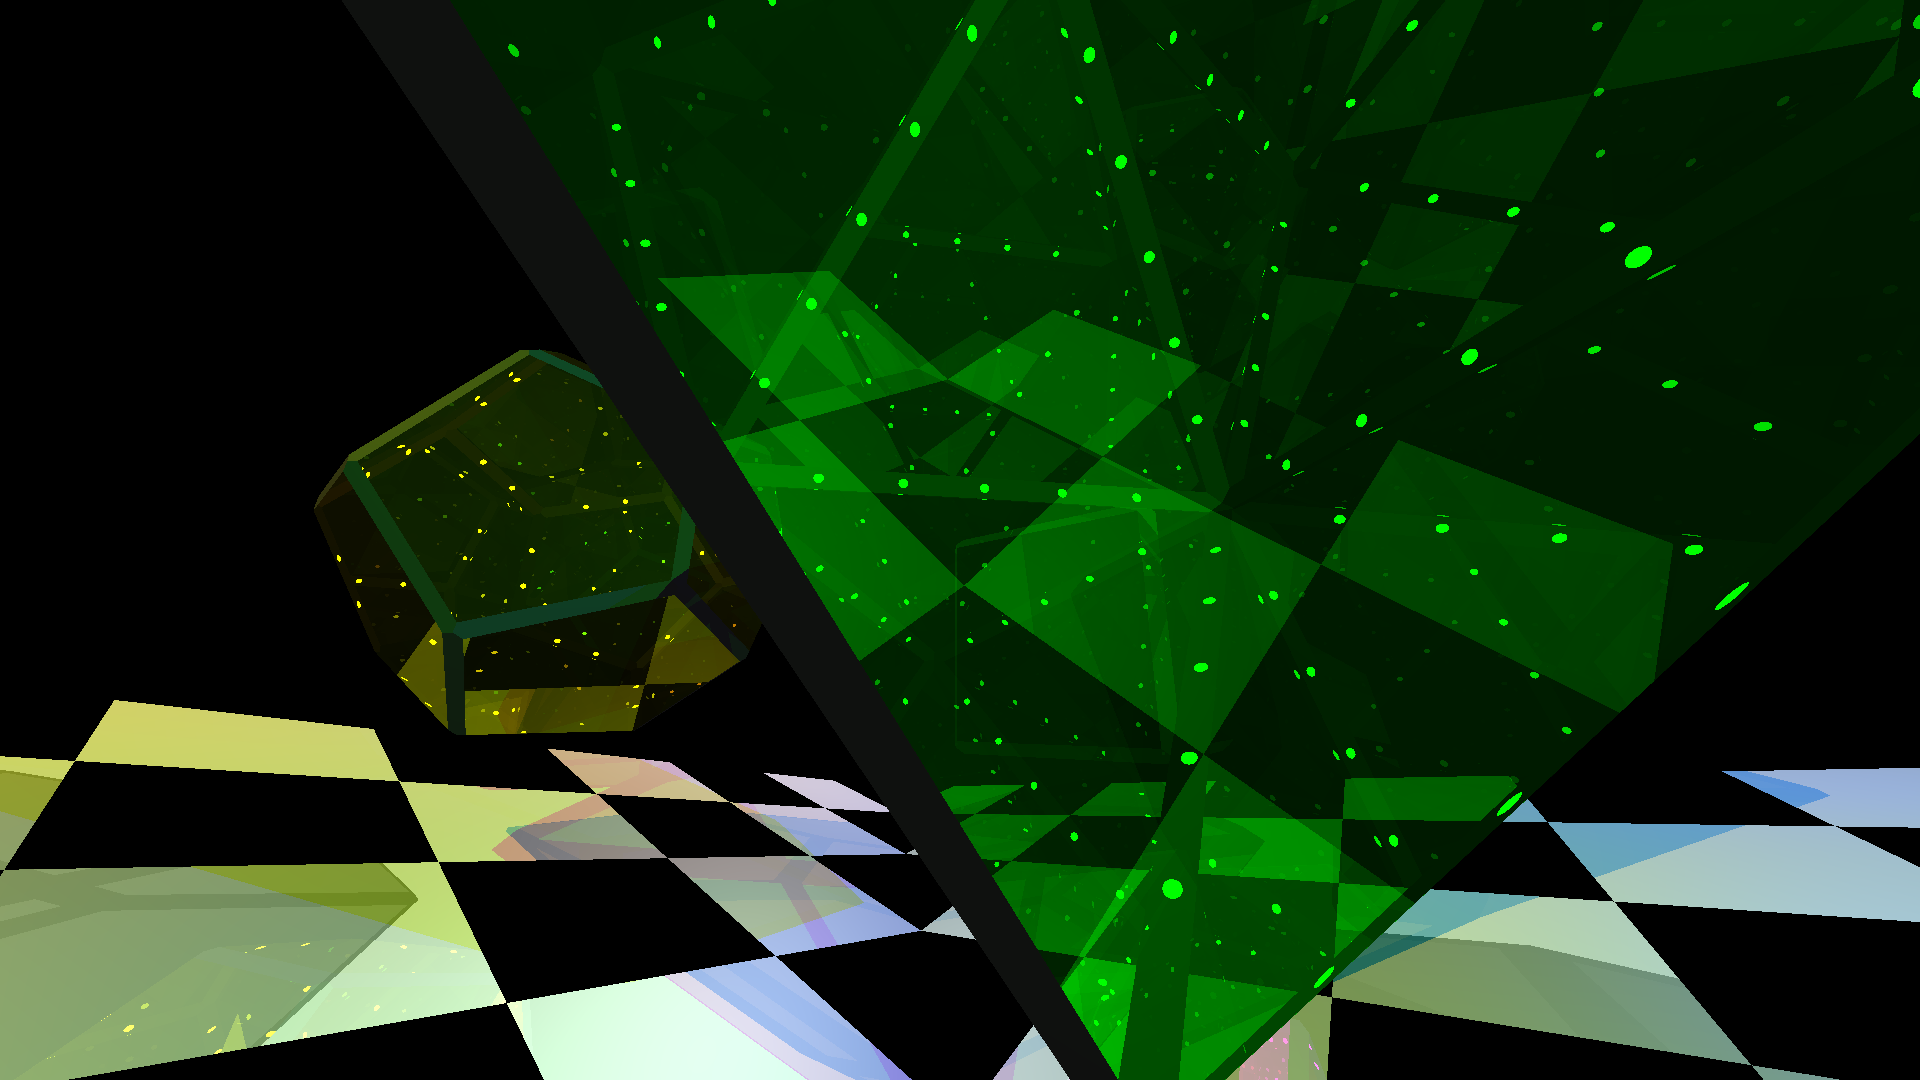
\includegraphics[width=\textwidth]{007.png}\newline\noindent
Эффект бесконечности в октаэдре
\end{center}
\begin{center}
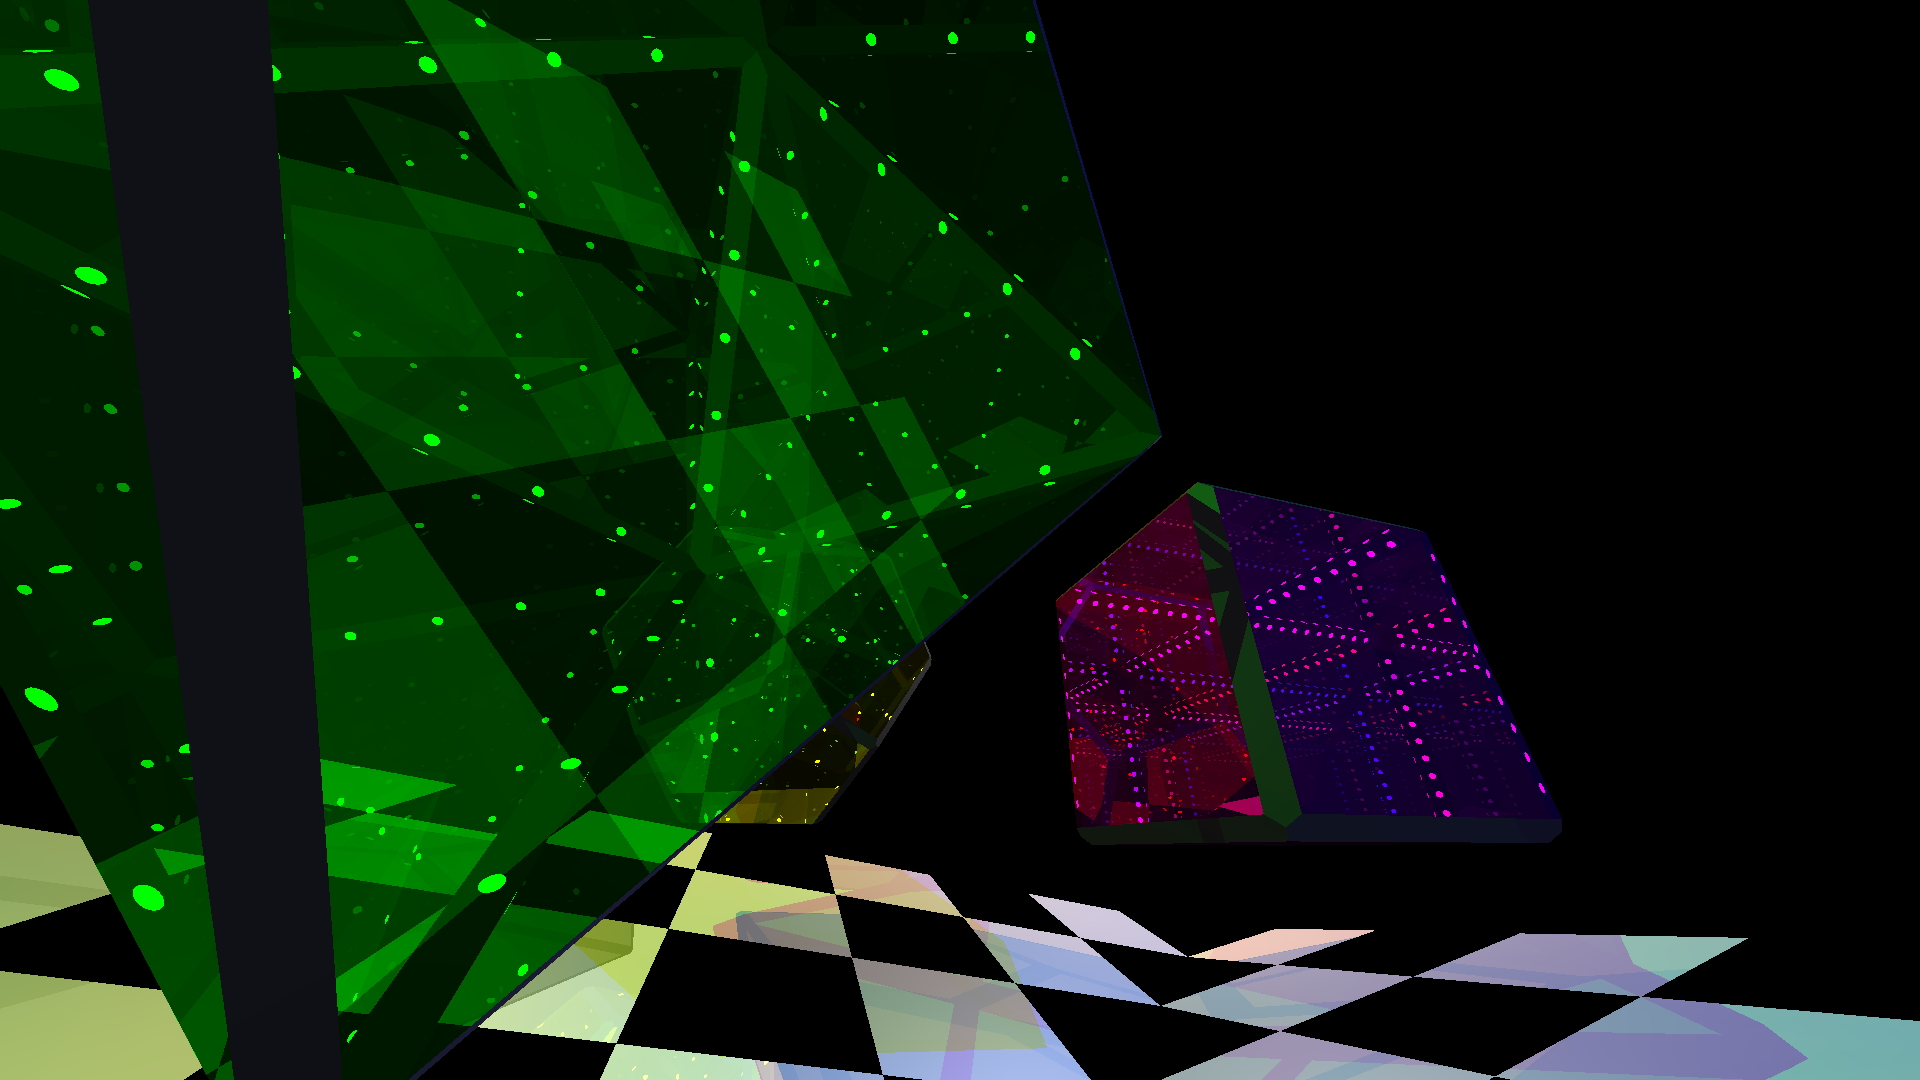
\includegraphics[width=\textwidth]{008.png}\newline\noindent
Додекаэдр частично виден сквозь октаэдр
\end{center}
\pagebreak

\begin{center}
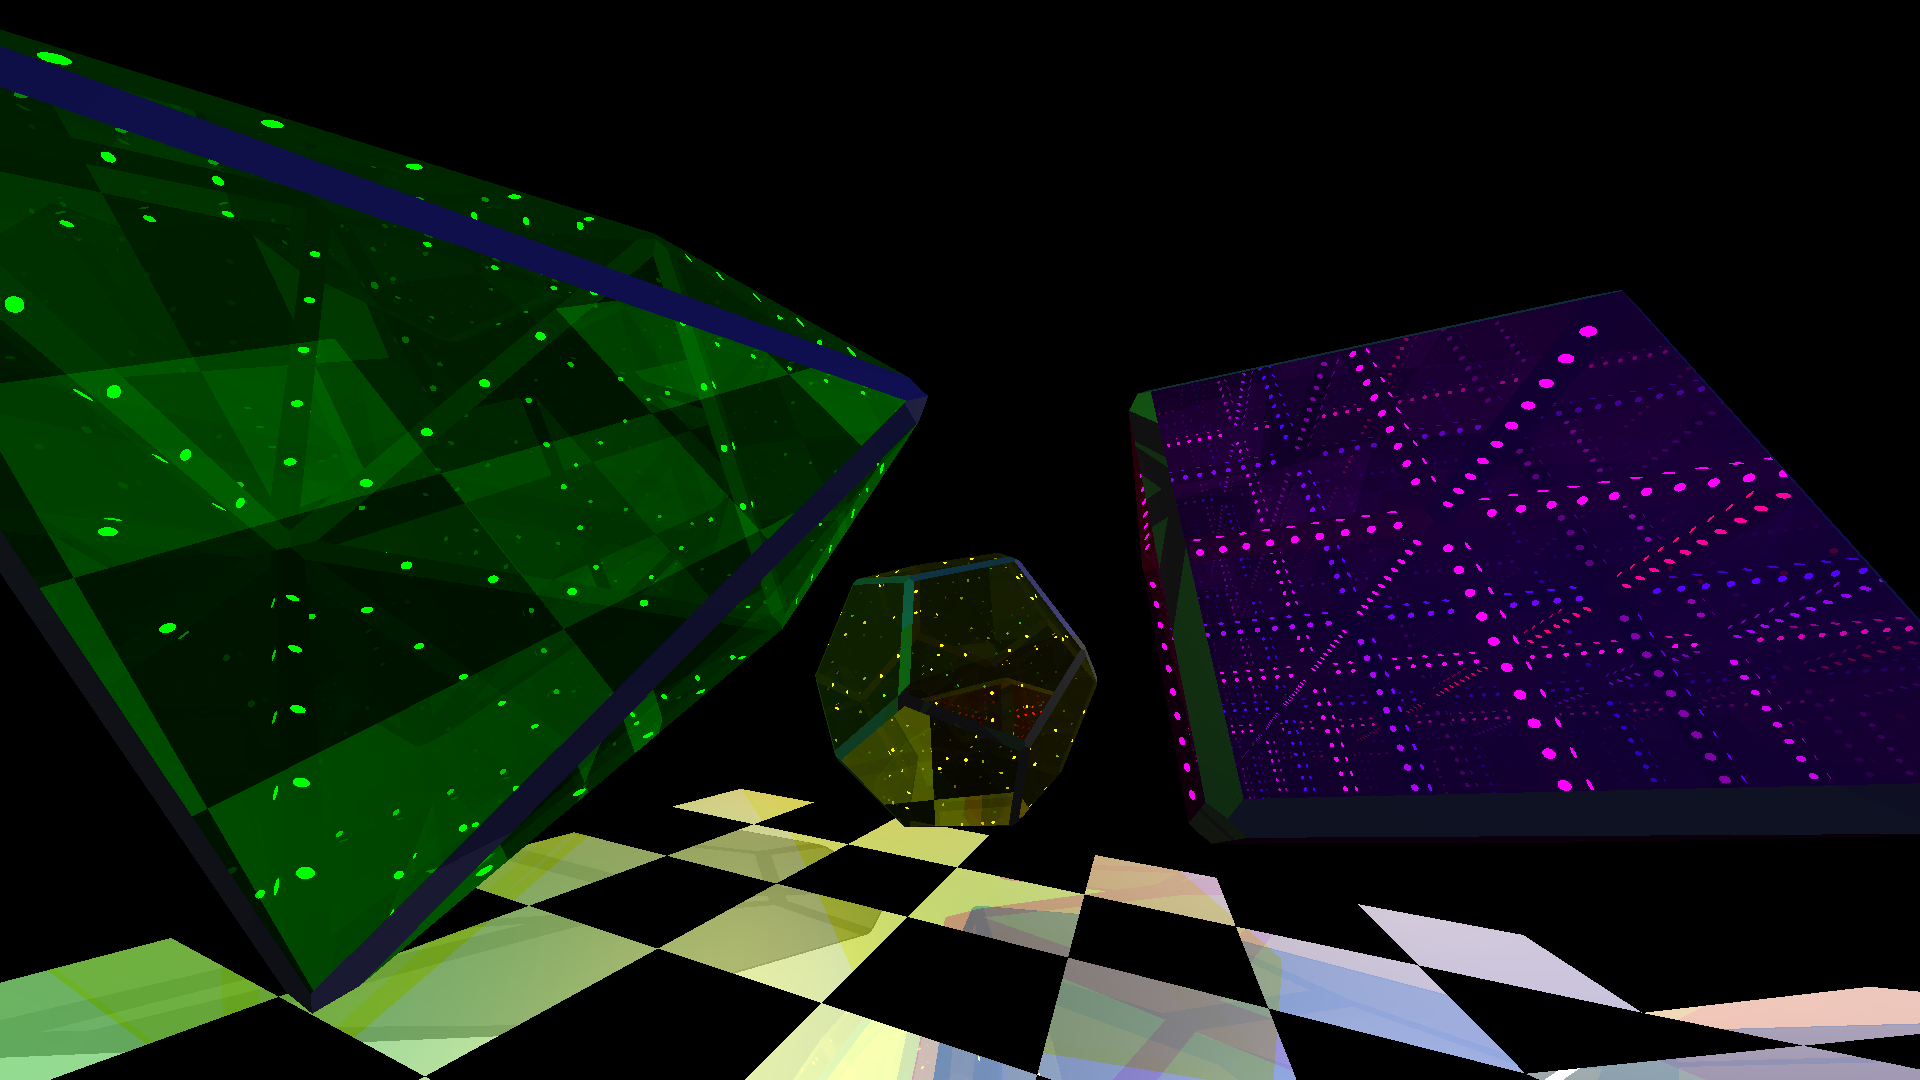
\includegraphics[width=\textwidth]{009.png}\newline\noindent
Все три фигуры
\end{center}
\begin{center}
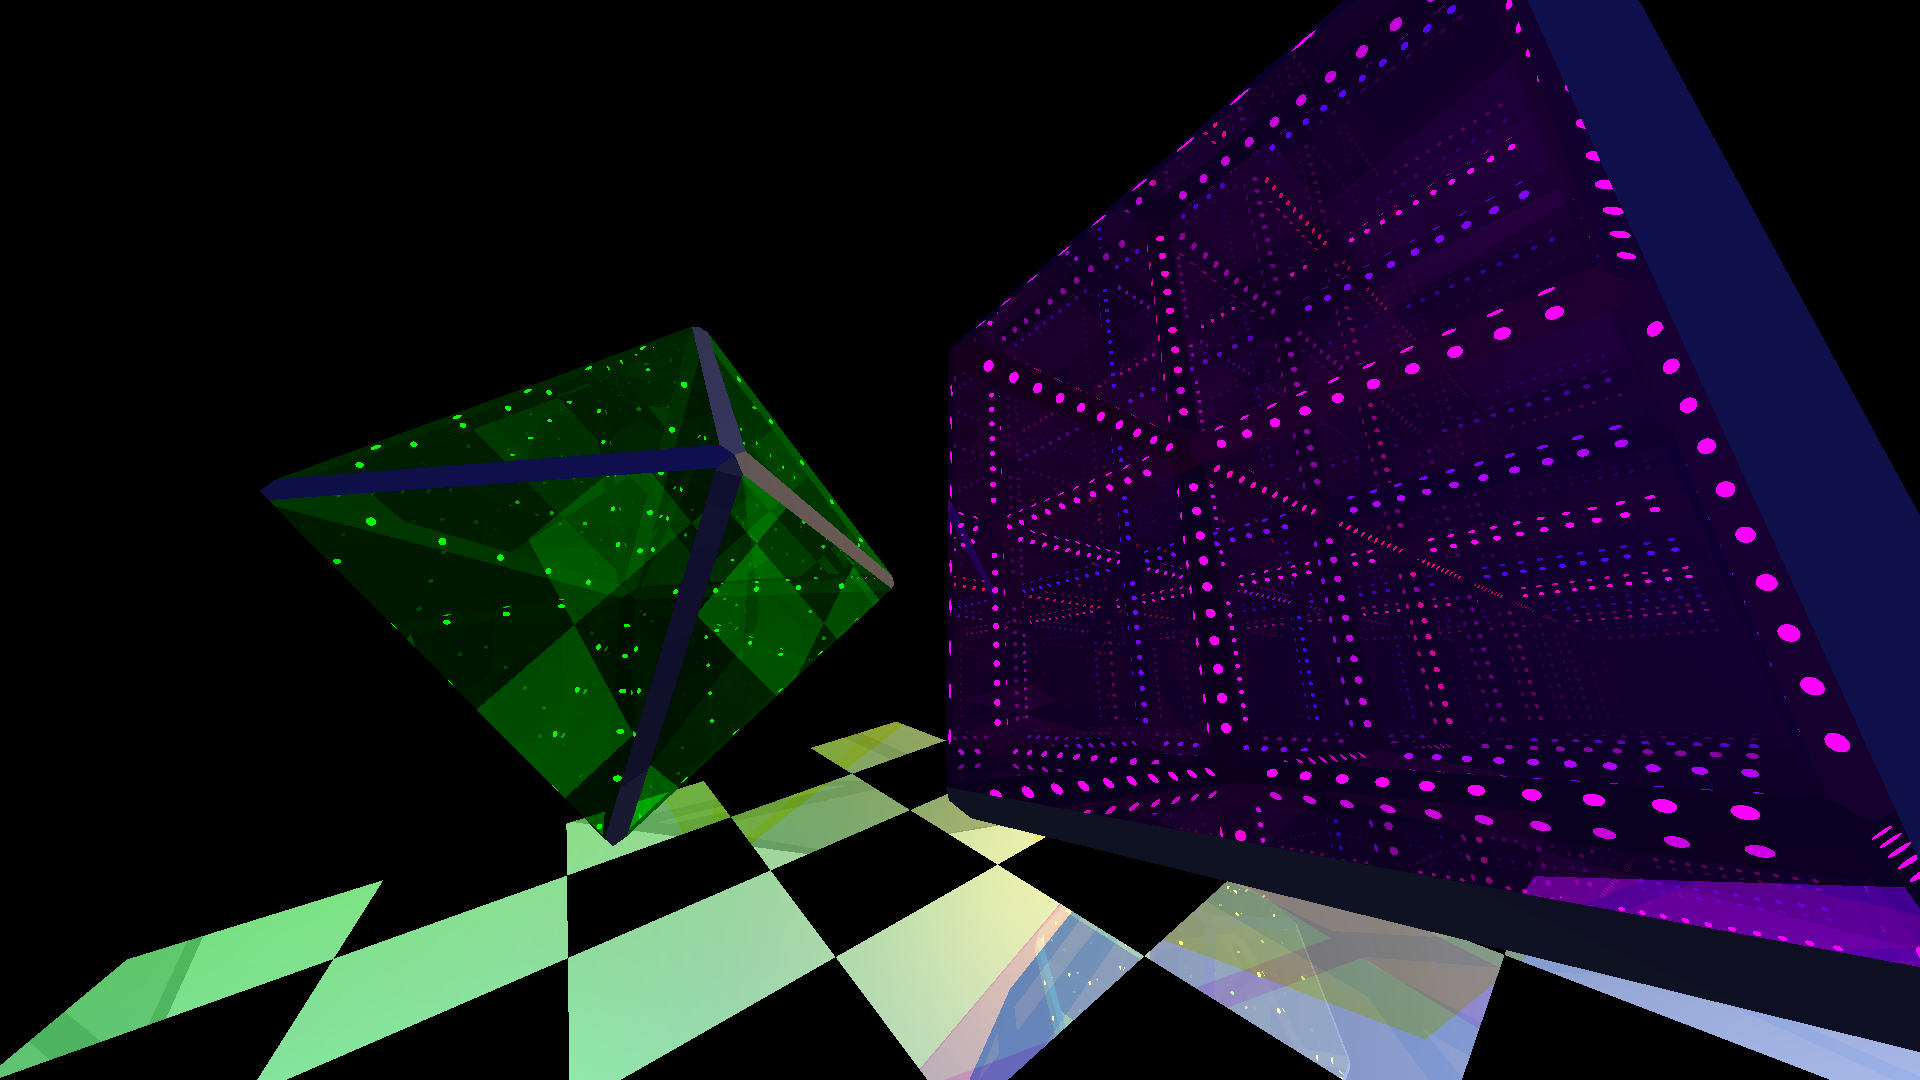
\includegraphics[width=\textwidth]{010.png}\newline\noindent
Эффект бесконечности в кубе с другого ракурса
\end{center}
\pagebreak
